\subsection{Labels Tab}
\label{sec:osgview_labels_tab} 
 
\begin{figure}[H]
   \center
    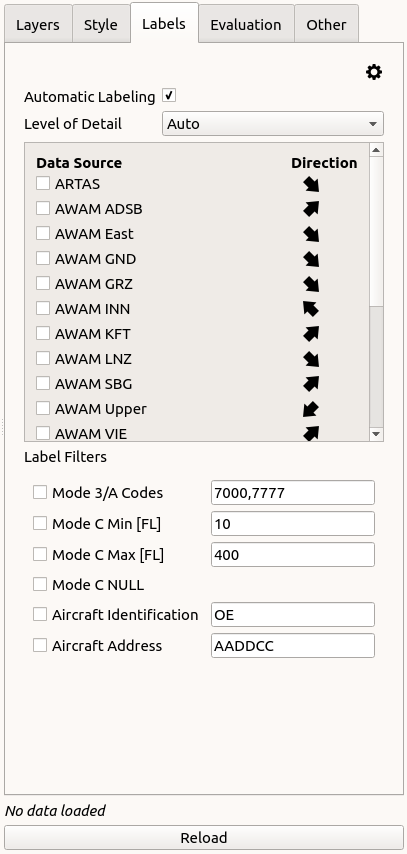
\includegraphics[width=8cm,frame]{figures/osgview_labels_tab.png}
  \caption{OSG View Labels tab}
\end{figure}

In the 'Labels' tab, several elements exist:

\begin{itemize}
 \item Layer Mode: Defines how layers are generated. Please refer to Section \nameref{sec:layer_mode} for details.
 \item Connect Last Layer: Whether grouped target reports in the last layer should be connected using lines
 \item Connect None Height: If groups are connected, whether target reports with not height information should be connected
 \item Blend Mode: Defines the drawing blend mode, allowing clearer symbols (contour) or colors (src-over).
 \item Style: Defines how geometry is styled. Please refer to Section \nameref{sec:style} for details.
 \item Render Order: Defines the drawing order of DBContents. To bottom one is drawn first, the top one last (over all others)
 \item Update button: Triggers a redraw or reload of the geometry, becomes available after a change if needed.
\end{itemize} 
